\documentclass[aspectratio=169]{../latex_main/tntbeamer}  % you can pass all options of the beamer class, e.g., 'handout' or 'aspectratio=43'
\usepackage{dsfont}
\usepackage{bm}
\usepackage[english]{babel}
\usepackage[T1]{fontenc}
%\usepackage[utf8]{inputenc}
\usepackage{graphicx}
\graphicspath{ {./figures/} }
\usepackage{algorithm}
\usepackage[ruled,vlined,algo2e,linesnumbered]{algorithm2e}
\usepackage{hyperref}
\usepackage{booktabs}
\usepackage{mathtools}

\usepackage{amsmath,amssymb}

\DeclareMathOperator*{\argmax}{arg\,max}
\DeclareMathOperator*{\argmin}{arg\,min}

\usepackage{amsbsy}
\newcommand{\vect}[1]{\bm{#1}}
%\newcommand{\vect}[1]{\boldsymbol{#1}}

\usepackage{pgfplots}
\pgfplotsset{compat=1.16}
\usepackage{tikz}
\usetikzlibrary{trees} 
\usetikzlibrary{shapes.geometric}
\usetikzlibrary{positioning,shapes,shadows,arrows,calc,mindmap}
\usetikzlibrary{positioning,fadings,through}
\usetikzlibrary{decorations.pathreplacing}
\usetikzlibrary{intersections}
\pgfdeclarelayer{background}
\pgfdeclarelayer{foreground}
\pgfsetlayers{background,main,foreground}
\tikzstyle{activity}=[rectangle, draw=black, rounded corners, text centered, text width=8em]
\tikzstyle{data}=[rectangle, draw=black, text centered, text width=8em]
\tikzstyle{myarrow}=[->, thick, draw=black]

% Define the layers to draw the diagram
\pgfdeclarelayer{background}
\pgfdeclarelayer{foreground}
\pgfsetlayers{background,main,foreground}

% Requires XeLaTeX or LuaLaTeX
%\usepackage{unicode-math}

\usepackage{fontspec}
%\setsansfont{Arial}
\setsansfont{RotisSansSerifStd}[ 
Path=../latex_main/fonts/,
Extension = .otf,
UprightFont = *-Regular,  % or *-Light
BoldFont = *-ExtraBold,  % or *-Bold
ItalicFont = *-Italic
]
\setmonofont{Cascadia Mono}[
Scale=0.8
]

\renewcommand{\ttdefault}{Cascadia Mono}

% scale factor adapted; mathrm font added (Benjamin Spitschan @TNT, 2021-06-01)
%\setmathfont[Scale=1.05]{Libertinus Math}
%\setmathrm[Scale=1.05]{Libertinus Math}

% other available math fonts are (not exhaustive)
% Latin Modern Math
% XITS Math
% Libertinus Math
% Asana Math
% Fira Math
% TeX Gyre Pagella Math
% TeX Gyre Bonum Math
% TeX Gyre Schola Math
% TeX Gyre Termes Math

% Literature References
\newcommand{\lit}[2]{\href{#2}{\footnotesize\color{black!60}[#1]}}

%%% Beamer Customization
%----------------------------------------------------------------------
% (Don't) Show sections in frame header. Options: 'sections', 'sections light', empty
\setbeamertemplate{headline}{empty}

% Add header logo for normal frames
\setheaderimage{
	% 
\includegraphics[height=\logoheight]{figures/TNT_darkv4.pdf}
	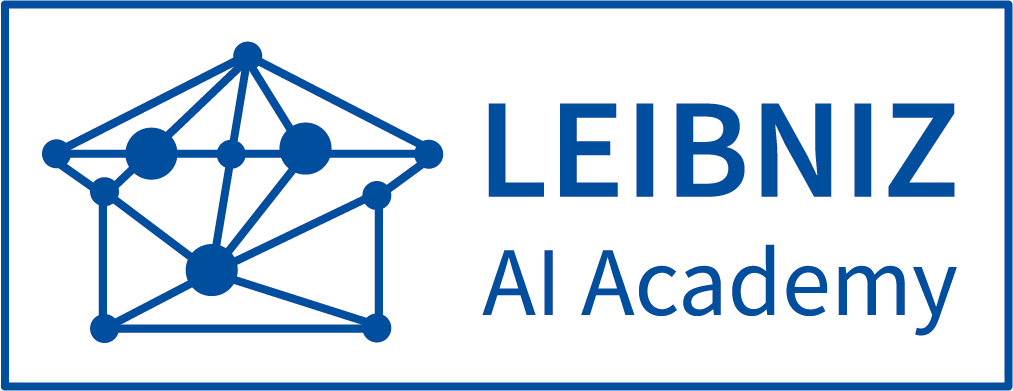
\includegraphics[height=\logoheight]{../latex_main/figures/Leibniz-AI-Academy_Logo}
	% 
\includegraphics[height=\logoheight]{figures/logo_tntluh.pdf}
}

% Header logo for title page
\settitleheaderimage{
	% 
\includegraphics[height=\logoheight]{figures/TNT_darkv4.pdf}
	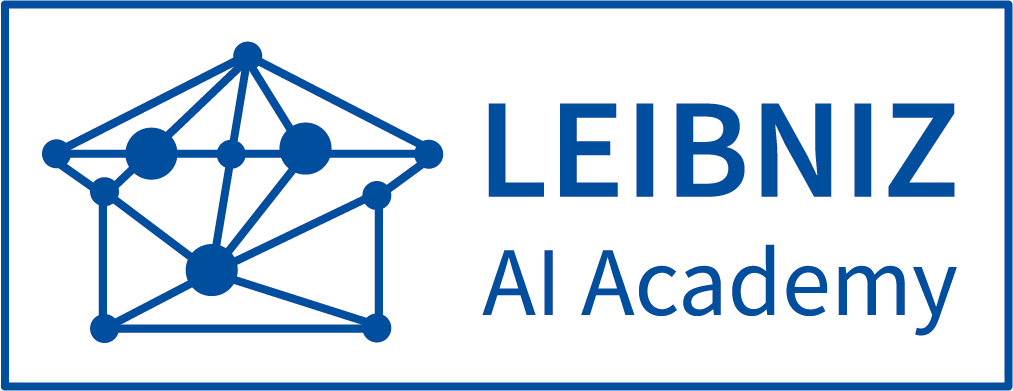
\includegraphics[height=\logoheight]{../latex_main/figures/Leibniz-AI-Academy_Logo}
	% 
\includegraphics[height=\logoheight]{figures/logo_tntluh.pdf}
}

% Title page: tntdefault 
\setbeamertemplate{title page}[tntdefault]  % or luhstyle
% Add optional title image here
%\addtitlepageimagedefault{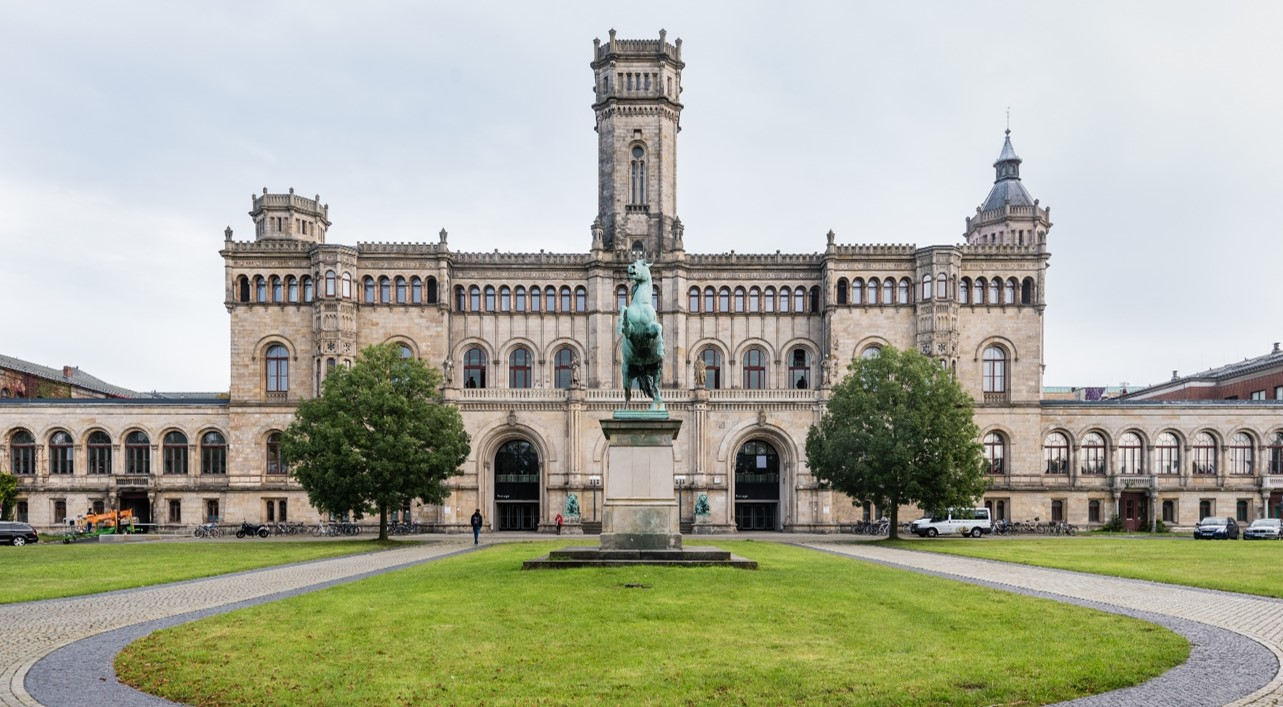
\includegraphics[width=0.65\textwidth]{figures/luh_default_presentation_title_image.jpg}}

% Title page: luhstyle
% \setbeamertemplate{title page}[luhstyle]
% % Add optional title image here
% \addtitlepageimage{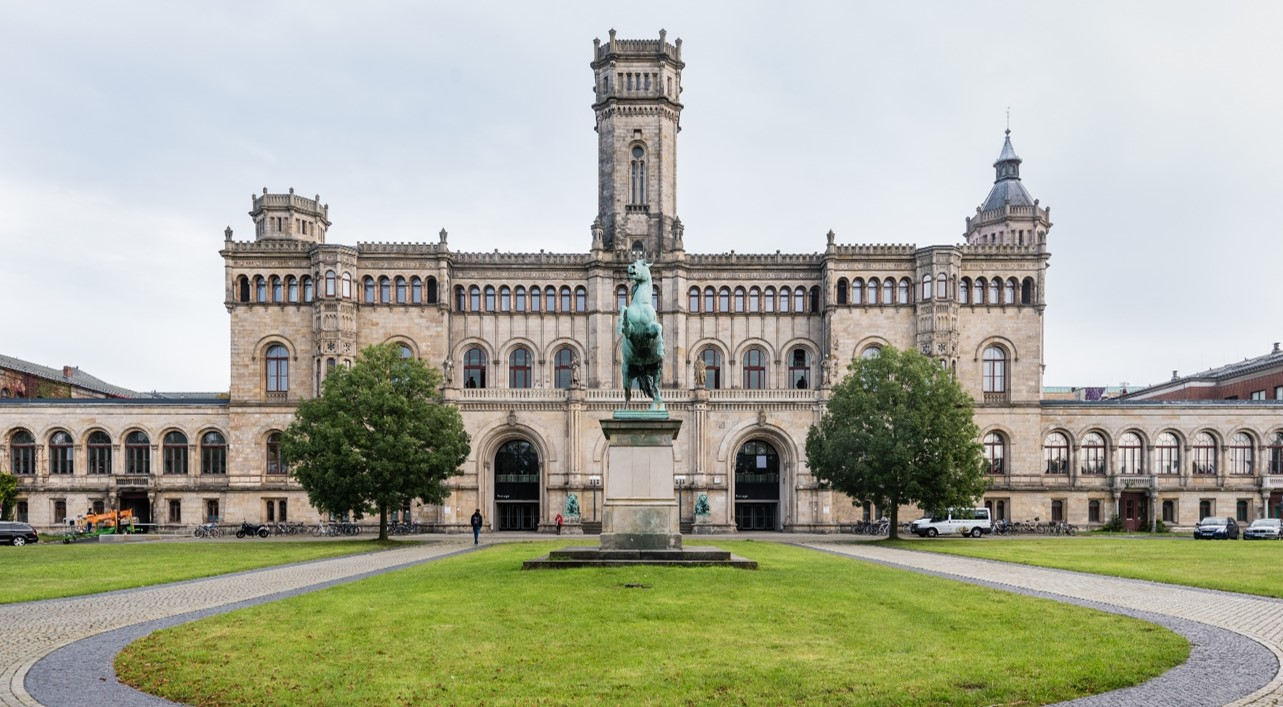
\includegraphics[width=0.75\textwidth]{figures/luh_default_presentation_title_image.jpg}}

\author[Abedjan \& Lindauer]{Ziawasch Abedjan \& \underline{Marius Lindauer}\\[1em]
	%
\includegraphics[height=\logoheight]{../latex_main/figures/luh_logo_rgb_0_80_155.pdf}\qquad
	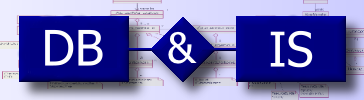
\includegraphics[height=\logoheight]{../latex_main/figures/DBIS_Kurzlogo.png}\qquad
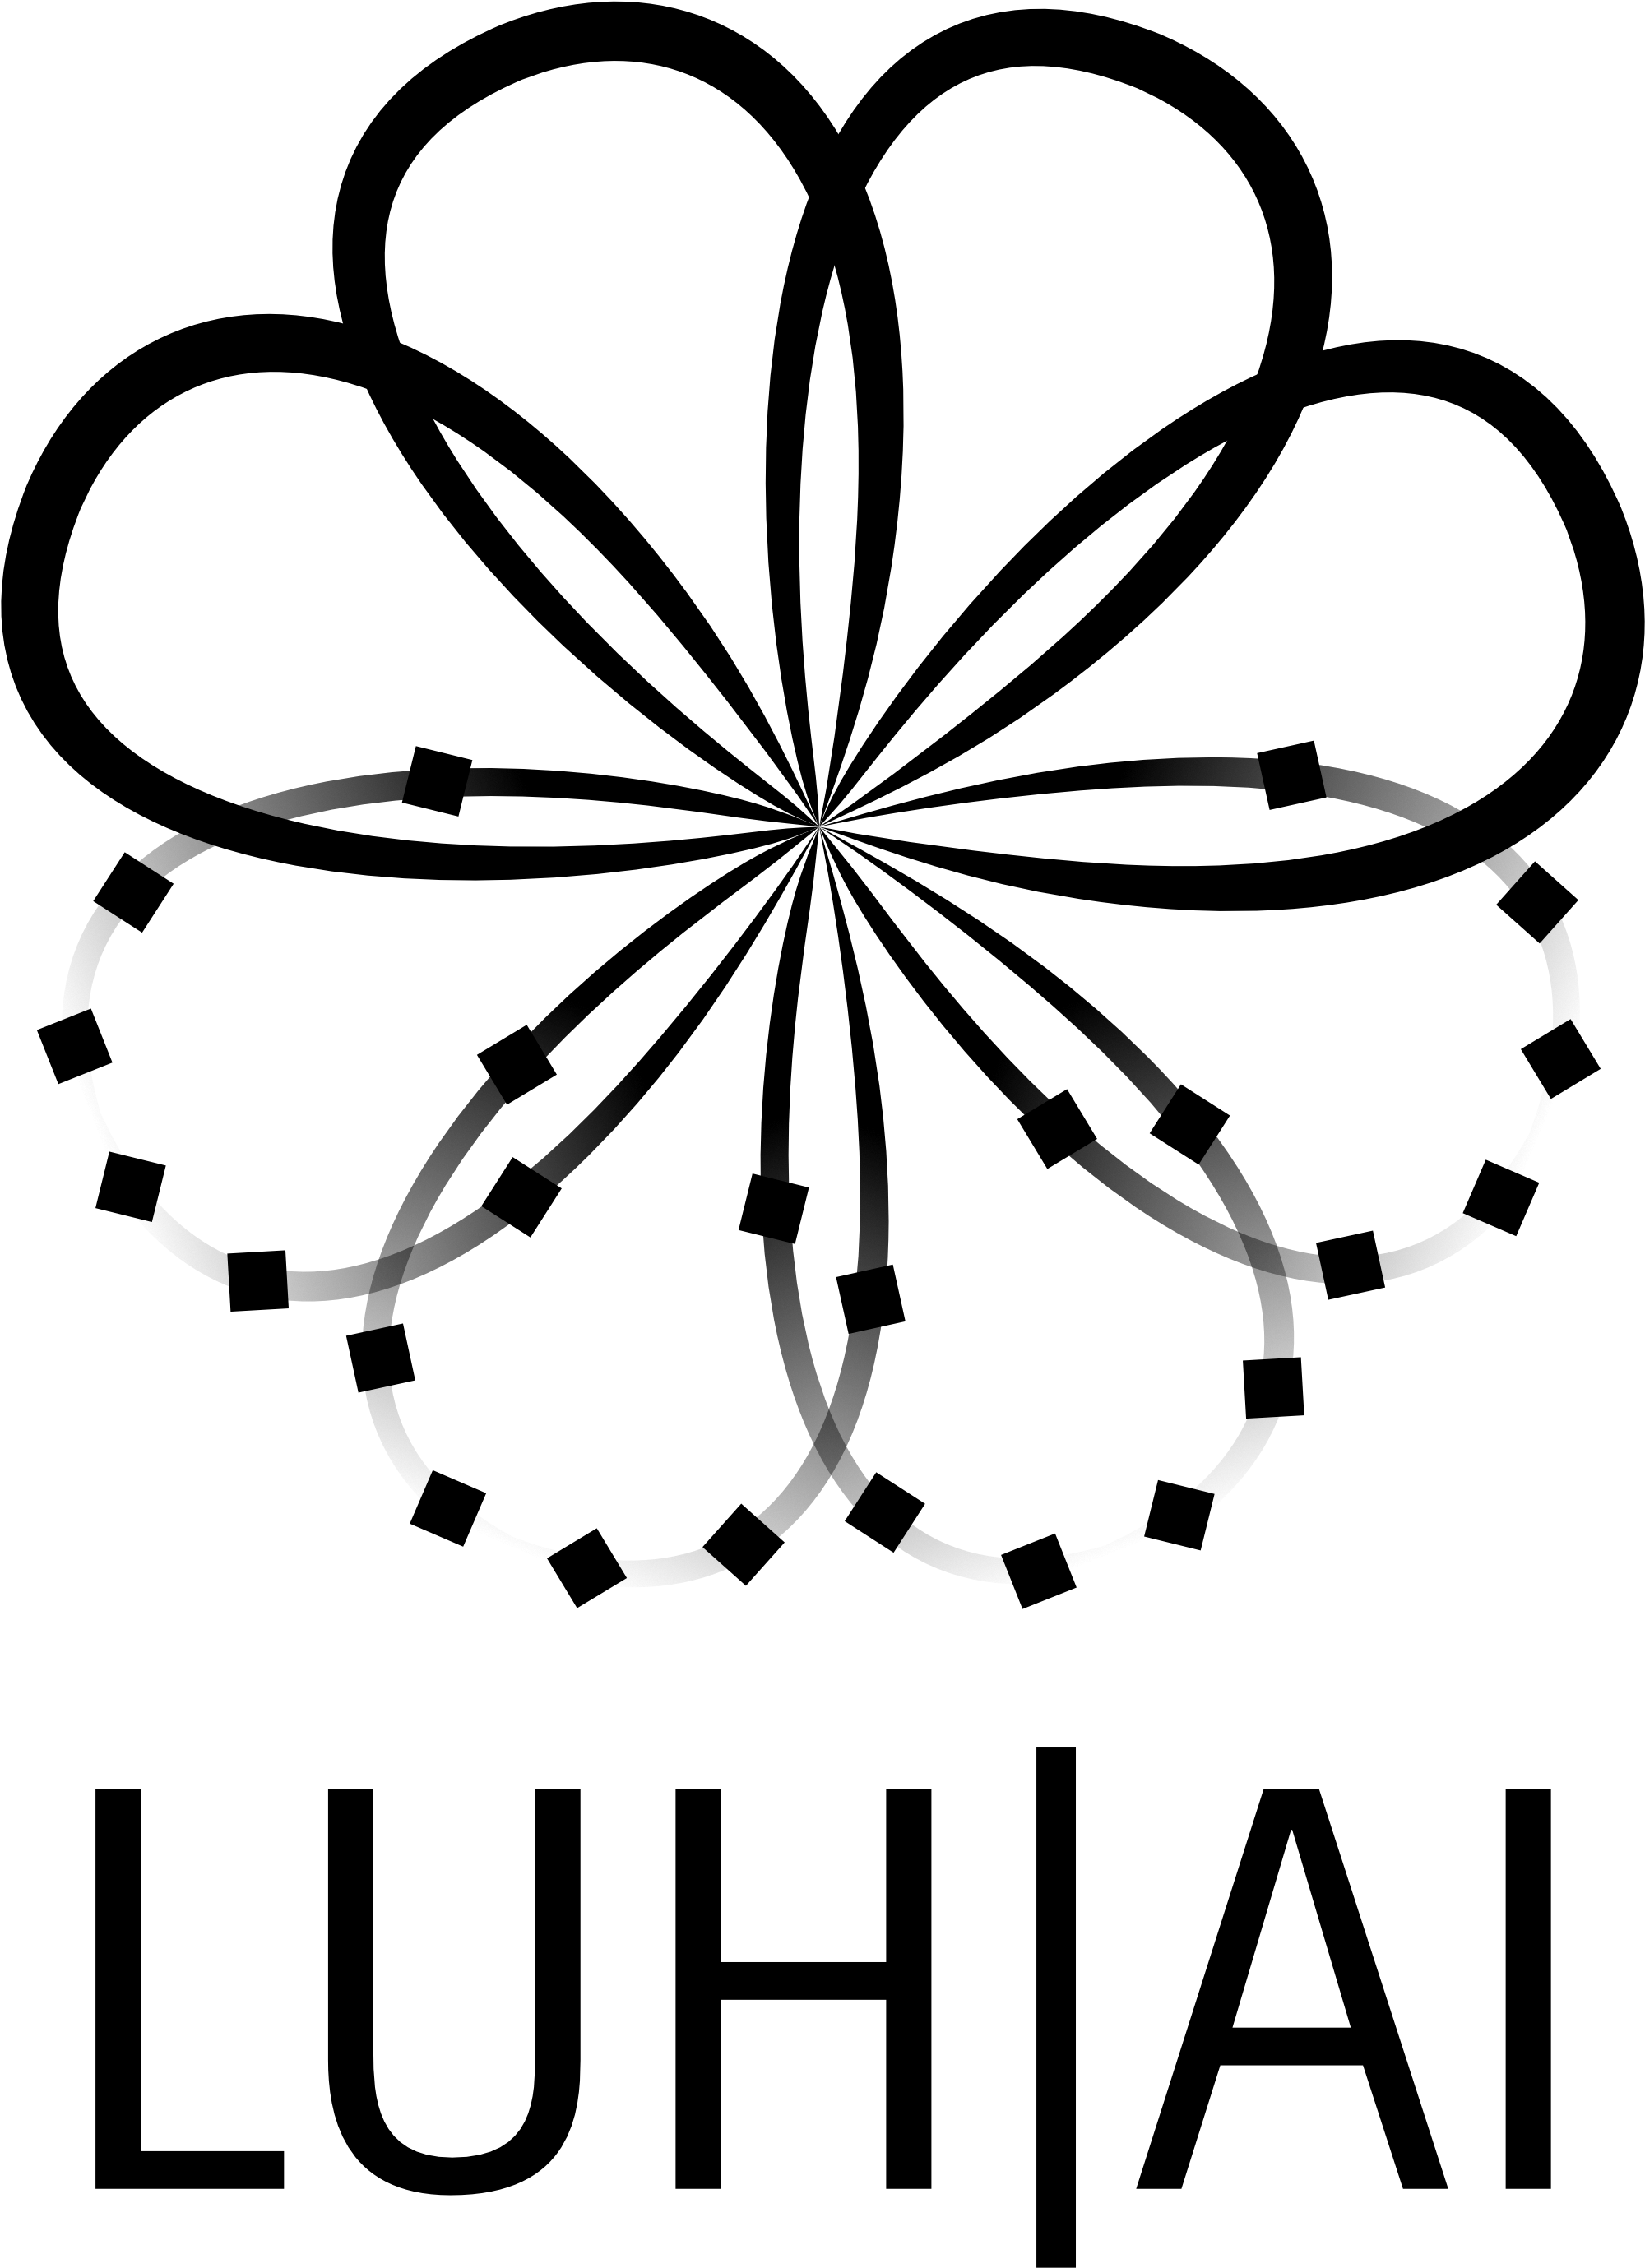
\includegraphics[height=\logoheight]{../latex_main/figures/logo_short_highres_black}\qquad
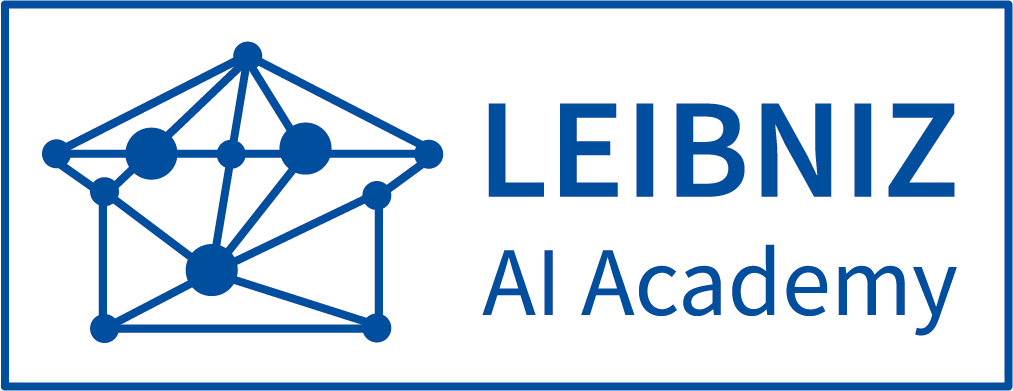
\includegraphics[height=\logoheight]{../latex_main/figures/Leibniz-AI-Academy_Logo}\qquad
%
\includegraphics[height=\logoheight]{../latex_main/figures/L3S.jpg}	
}
\date{\hspace{0.5em} {
\includegraphics[height=1.5em]{../latex_main/figures/Cc-by-nc-sa_icon.svg.png}}; extension of \href{https://ds100.org/fa21/}{[DS100]}
}


%%% Custom Packages
%----------------------------------------------------------------------
% Create dummy content
\usepackage{blindtext}

% Adds a frame with the current page layout. Just call \layout inside of a frame.
\usepackage{layout}


%%% Macros
%\renewcommand{\vec}[1]{\mathbf{#1}}
% \usepackage{bm}
%\let\vecb\bm

\title[DL: DL Operations]{DS: Deep Learning}
\subtitle{DL Operations}

\date{\hspace{0.5em} {
\includegraphics[height=1.5em]{../latex_main/figures/Cc-by-nc-sa_icon.svg.png}}}

\graphicspath{ {./figure/} }
%\institute{}


\begin{document}
	
	\maketitle

    \begin{frame}{Operations for DL}
        \begin{itemize}
            \item Besides, a simple flow of data through neurons, there are further important operators in neural networks
            \item In principle, DNNs are universal function approximations, but in practice, these operations help efficiently train DNNs
            \item Note that with using these operators you add a certain kind of inductive bias (i.e., how should the model being learned) or regularization 
        \end{itemize}
    \end{frame}
 
    \begin{frame}
    \frametitle{Convolution Operation}
    \vspace*{-2em}
    \begin{itemize}
        \item Convolution is a fundamental operation in CNNs (Convolutional Neural Networks).
        \item It involves a filter (or kernel) that slides over the input feature map and computes dot products.\footnote{In a 2d-Conv, this refers actually to a element-wise multiplication (or a flattened representation to a vector) and not to a real dot product. The dot-product operation is relevant for 3d-Convs (for which we take the channels into account).}
        \item Typically, used for images
    \end{itemize}
    \begin{equation}
        (I * K)(i,j) = \sum_{m}\sum_{n} I(i-m,j-n)K(m,n)
    \end{equation}
        \centering
            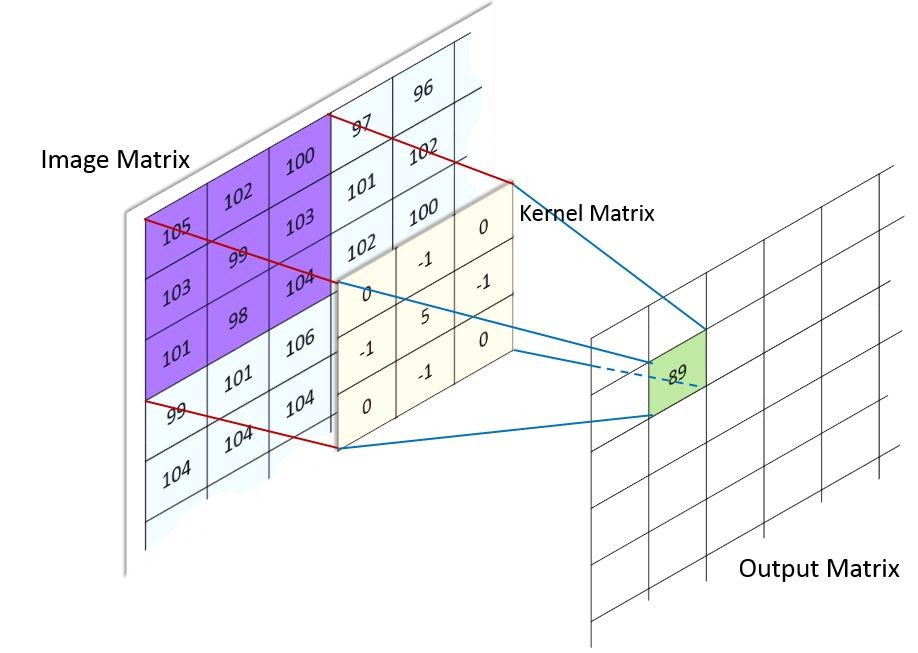
\includegraphics[width=0.33\textwidth]{figure/convolution.jpg}
        Credit: [\href{https://www.linkedin.com/pulse/image-processing-convolution-filters-calculation-gradients-yadav/}{Yadav 2023}]
    \end{frame}
    
    \begin{frame}
    \frametitle{Convolution Parameters}
    \begin{itemize}
        \item \textbf{Stride:} Determines the step size of the filter as it slides over the input.
        \item \textbf{Padding:} Controls the spatial size of the output. Common types are 'valid' (no padding) and 'same' (zero-padding).
        \item \textbf{Depth:} Number of filters applied. Each filter generates a separate output channel.
    \end{itemize}
    \end{frame}

    \begin{frame}
    \frametitle{Pooling Operation}
    \begin{itemize}
        \item Pooling reduces the spatial dimensions (width and height) of the input volume.
        \item Common types are \textbf{Max Pooling} and \textbf{Average Pooling}.
    \end{itemize}
        \centering
        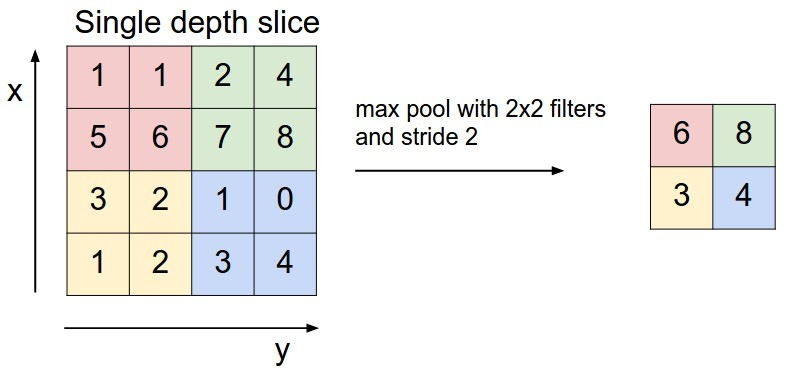
\includegraphics[width=0.6\textwidth]{figure/maxpool.jpeg} Credit: [\href{https://cs231n.github.io/convolutional-networks/#overview}{cs231n}]
    \end{frame}
    
    \begin{frame}
    \frametitle{Types of Pooling}
    \begin{itemize}
        \item \textbf{Max Pooling:} Takes the maximum value from the portion of the image covered by the filter.
        \item \textbf{Average Pooling:} Takes the average value from the portion of the image covered by the filter.
    \end{itemize}
    \begin{equation}
        y(i,j) = \max_{m,n} x(i+m,j+n) \quad \text{(Max Pooling)}
    \end{equation}
    \begin{equation}
        y(i,j) = \frac{1}{mn}\sum_{m,n} x(i+m,j+n) \quad \text{(Average Pooling)}
    \end{equation}
    \end{frame}
    
    \begin{frame}
    \frametitle{Batch Normalization}
    \begin{itemize}
        \item Batch normalization is used to normalize the input of each layer.
        \item It helps in speeding up training and providing some regularization.
    \end{itemize}
    \begin{equation}
        \hat{x}^{(k)} = \frac{x^{(k)} - \mu^{(k)}}{\sqrt{(\sigma^{(k)})^2 + \epsilon}}
    \end{equation}
    \begin{equation}
        y^{(k)} = \gamma^{(k)} \hat{x}^{(k)} + \beta^{(k)}
    \end{equation}
    \begin{itemize}
        \item \(\mu^{(k)}\) and \(\sigma^{(k)}\) are the mean and variance of the batch.
        \item \(\gamma^{(k)}\) and \(\beta^{(k)}\) are learnable parameters.
    \end{itemize}
    \end{frame}
    
    \begin{frame}
    \frametitle{Benefits of Batch Normalization}
    \begin{itemize}
        \item Reduces internal covariate shift.
        \item Allows for higher learning rates.
        \item Acts as a form of regularization.
    \end{itemize}
    \end{frame}
    
    \begin{frame}
    \frametitle{Dropout}
    \begin{itemize}
        \item Dropout is a regularization technique used to prevent overfitting.
        \item During training, randomly selected neurons are ignored (dropped out).
        \item Note: Learning curves will become dumpy
    \end{itemize}
    \begin{equation}
        y_i = 
        \begin{cases} 
        0 & \text{with probability } p \\
        \frac{x_i}{1-p} & \text{with probability } 1-p 
        \end{cases}
    \end{equation}

    \centering
    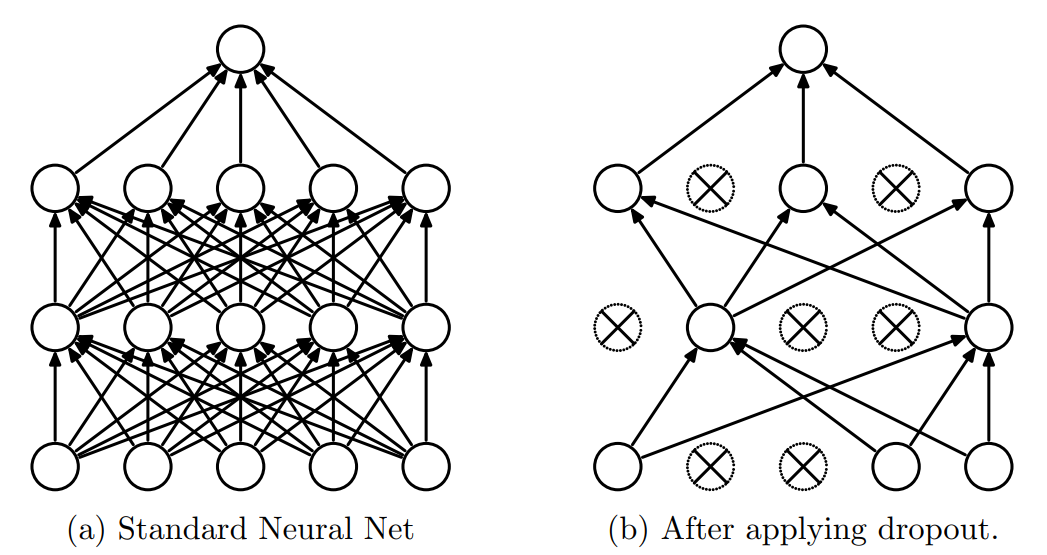
\includegraphics[width=0.45\textwidth]{figure/dropout.png} Credit: [\href{https://jmlr.org/papers/volume15/srivastava14a/srivastava14a.pdf}{Srivastava et al. 2015}]

    \end{frame}
    
    \section{Summary}
    \begin{frame}
    \frametitle{Summary}
    \begin{itemize}
        \item Convolution, batch normalization, pooling and dropout are key operations in deep neural networks.
        \item Convolution captures spatial hierarchies, batch normalization stabilizes learning, pooling reduces dimensionality and dropout prevents overfitting.
        \item Understanding these operations is crucial for designing effective neural network architectures.
    \end{itemize}
    \end{frame}

    


 	
\end{document}